% Documentclass options:
%    10pt, 11pt, 12pt  -- set type size
%    draft             -- single space, mark overfull hboxes on paper
%    final             -- double space, don't mark overfull hboxes on paper
%    oneside           -- format for one-sided printing
%    twoside           -- format for two-sided printing
% Defaults are 11pt,final,oneside.  Keep these, please.
\documentclass[11pt]{ucscthesisbs}
\bibliographystyle{apalike2}
\usepackage{natbib}
\usepackage{graphicx,epsf}% Include figure files


% The following declaration is for citations and bibliographies consistent with
% Astrophysical Journal specifications.  It may be left out or replaced with
% another bibliography/citation style.  See also the "\bibliographystyle"
% command later in this file.
%\usepackage{apj}

\usepackage{xcolor}
\usepackage{pagecolor}
\usepackage{lipsum}  
\usepackage{subfig}
\usepackage{amsmath}
\usepackage[font=small,labelfont=bf]{caption}

% \pagecolor{darkgray}
% \color{white}

\pagecolor{white}
\color{black}


\begin{document}

% Declarations for Front Matter

\title{Thermal Evolution of Uranus and Neptune with Condensation-inhibited Convection}
\author{Robert Schroder}
\degreeyear{2020}
\degreemonth{November}
\degree{BACHELOR OF SCIENCE}
\field{ASTROPHYSICS}%
% Declare up to five committee members.  The text will be reproduced directly
% on the signature page.  Though the chair is a committee member, leave
% him/her out of the \committeemember declarations.  Make sure \numberofmembers
% agrees with the number of committee members declared INCLUDING the chair.
% If it is wrong, you will get extra or missing lines on the signature page.
%
\chair{Bruce Schumm}
\thesisadvisor{Christopher Mankovich}
\technicaladvisor{Jonathan Fortney}
\numberofmembers{2}




\campus{Santa Cruz}

\maketitle
\copyrightpage

\begin{frontmatter}

\begin{abstract}
This will be the last section written, once we have finished our results and conclusion.
\end{abstract}

\tableofcontents
%
% The most recent (10/95) guidelines make absolutely no mention of the list
% of figures and list of tables.  Are they necessary?  If not, comment the
% next two lines out.
%
\listoffigures
\listoftables

\begin{dedication}
\null\vfil
{\large
\begin{center}
To Who,\\\vspace{12pt}
M  ention to who, if anyone, here
\end{center}}
\vfil\null
\end{dedication}

\begin{acknowledgements}
I'd like to thank....
\end{acknowledgements}


\end{frontmatter}

%\part{First Part}

\chapter{Introduction}
Giant planets radiate away their latent heat of formation through the top of their atmosphere. If they cool to a point where the amount they radiate away is equal to the amount of radiation they receive from their parent star, they enter thermal equilibrium with their surroundings. At the present time, the giant planets in our solar system: Saturn, Jupiter, and Neptune, all have effective temperatures greater than their equilibrium temperature, an intrinsice heat source, except for Uranus. Observations of Uranus show a planet that appears to be in thermal equilibrium with its parent star, a planet with no intrinsic temperature, cooler than its more distant neighbor, Neptune, a planet of similar mass and composition. Thermal evolution models for Uranus have not matched observation, instead predicting a warmer effective temperature at $4.6$ Gyr, the current age of the solar system.\citep{fortney_2011}, \citep{podolak_1991}, \citep{hubbard_1995}, \citep{scheibe_2019} [There are other papers by Nettelmann 2013, Linder 2019 that I haven't looked at yet]. 

There have been various attempts to explain Uranus' cool temperature. Early investigations posited that a stratified interior, possibly stable against convection, would allow heat to be trapped deep within the the interior.\citep{podolak_1991}. Later work built on this idea, investigating the formation of stable condensation zones\citep{friedson_2017}, \citep{leconte_2017}, and \citep{guillot_1995}, and thermal boundary laters\citep{nettelmann_2016}, that would inhibit convection . It was speculated that the presence of these condensation zones could trap heat deep within the interior, allowing the envelope above to cool more rapidly, thereby lowering the planet's effective temperature.

In this paper, we investigate whether stable water condensation zones form within in the interiror of Uranus and Neptune, and present their potential impact on the thermal evolution of the these planets.
...
We use the model described in chapter 2.1 as our baseline...
The specifics of our model is described in chapter 2.2.

\chapter{Model}

\section{Historical Work}
The physics of the interior structure of the solar system gas and ice giants, and attempts to model their thermal evolution, date back to the mid to late twentieth century, after the first observation of Jupiter's instrinsic temperature by \cite{low_1966}, with subsequent investigations into the theory of giant planet structure and evolution\citep{hubbard_1977}, \citep{hubbard_1977_2}, \citep{podolak_1991}. We begin with a description of the physics of our baseline structure model, starting with the conservation of mass:

\begin{equation}
  \frac{dm}{dr} =4 \pi r^{2}\rho  
\end{equation}
where $dm$ is the mass contained within a sphere of radius $r$, and $\rho(r)$ is the density at radius $r$. Hydrostatic equilibrium is also assumed and described by:

\begin{equation}
  \frac{dP}{dr} = -\frac{Gm\rho}{r^{2}}  
\end{equation}
where $P$ is the pressure and $G$ is the gravitational constant. 


\section{Three-layer Model with Dry Adiabat}
We employ a three-layer interiror structure, seen schematically in Figure 2.1. At the center of the planet is a core made of rock and ice. Moving outward, the inner envelope is $H_{2}O$ dominated, with uniform concentrations of $H$, $He$, and $H_{\rm{2}}O$. We use the MAZEVET equation of state (EOS) \citep{mazevet_2019} to define the structure of the inner envelope. The outer envelope, below 10 bars, contains trace amounts of $H_{\rm{2}}O$, but is mostly $H$ and $He$, dominated, and utilizes the MH13SCVH EOS \citep{miguel_2018}. 

Historically, interior structure models have assumed that the interiors are composed of compressible gasses that are statically unstable and fully convective. In a dry-convective model such as this, a parcel of gas rises as its temperature increases while its pressure remains constant. This process happens without the addition or loss of heat from the parcel, a process referred to as adiabatic. Furthermore, while there may be a critical concentration for a condensible species, all this dry model does not allow for condensation. The temperature-pressure profile follows a dry adiabat gradient\citep{kippenhahn_2012}, given by :

\begin{equation}
\nabla_{\rm ad} = \left( \frac{\partial \ln T}{\partial \ln P} \right)_{\rm s}
\end{equation}

\begin{figure}[ht!]
 \centerline{
  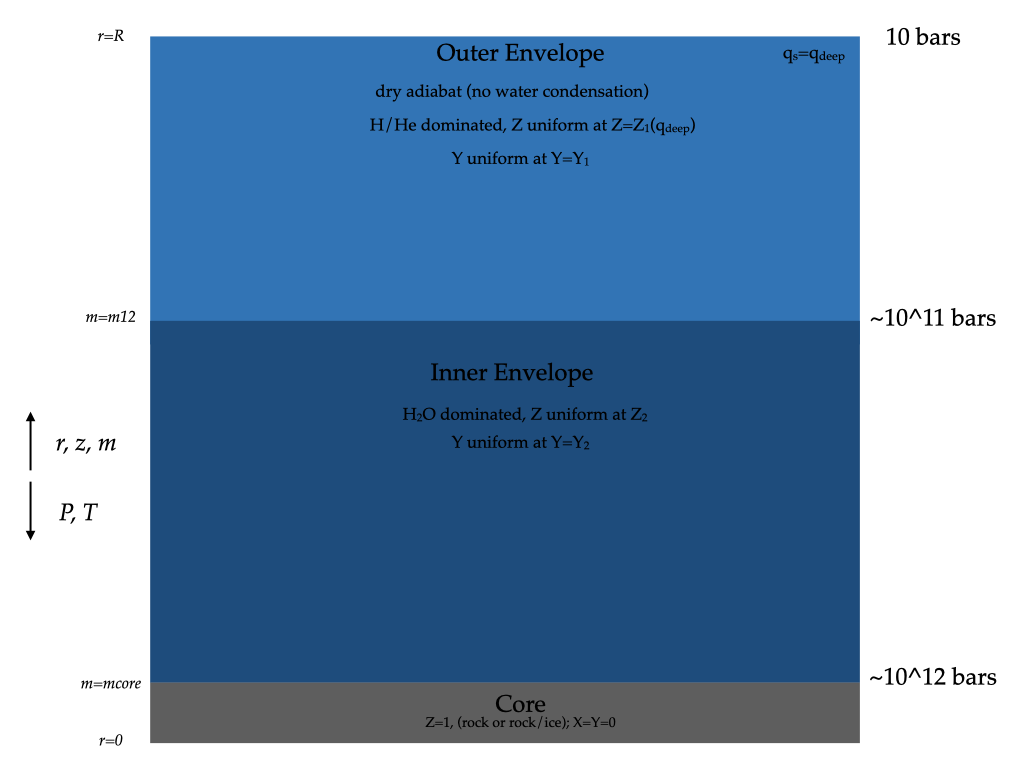
\includegraphics[width=6.0in]{figures/structure_schematic_images/structure_schematic_images.001.png}
 }
\caption[A Standard Interior Structure Model]
{The structure for a fully convective, dry adiabatic interior. In this model, the inner and outer envelopes are assumed to be well mixed, fully convective, and following a dry adiabat. The core is composed of rock and ice. The inner envelope is water dominated, with with uniform concentrations of hydrogen, helium, and water; whereas, the outer envelope is hydrogen and helium dominated, with trace amounts of water. The 'atmosphere' exists above 10 bars.}
\label{fig:standard_dry_interior}
\end{figure}

Finally, beyond the outer envelope is the atmosphere. When modeling the thermal evolution of gas and ice giants, it has long been recognized that model atmospheres constitute an outer boundary condition for interior structure models, providing key inputs that impact cooling times for interior structure models. Our work considers both \citep{graboske_1975} and \citep{fortney_2011} model atmospheres. Unless otherwise stated, our results will utilize the Fortney 2011 model atmospheres. 

\section{Inclusion of Moist Adiabat Within Outer Envelope}
Our interior structure model departs from the standard model described above by adding a moist adiabatic layer to the outer envelope that, under favorable conditions, allows for the condensation of $H_{2}O$. Gases condense at at sufficiently low temperatures or high pressures(cite pierrehumbert). Condensation of a gas is characterized by its saturation vapor pressure, $P_{\rm sat}$, given by: 

\begin{equation}
  P_{\rm sat}(T) = P_{\rm sat}(T_{\rm 0})e^{-\frac{1}{R_{\rm gas}}\big(\frac{1}{T}-\frac{1}{T_{\rm 0}}\big)}
\end{equation}

where $R_{\rm gas}$ is the gas constant for the condensible species. When the partial pressure of a gas, $P_{\rm gas}$, is less than $P_{\rm sat}$, the parcel of gas is 'unsaturated'. When $P_{\rm gas} = P_{\rm sat}$, the gas is 'saturated'. And, when $P_{\rm gas} > P_{\rm sat}$, the parcel is 'supersaturated'. Each condensible species has its own saturation vapor pressure.

The condensation of water in the interior of hydrogen-dominated atmospheres has some notable differences with our experience of water condensation within our own planet's atmosphere \citep{leconte_2017} \citep{friedson_2017} \citep{guillot_2019} \citep{guillot_1995}. On Earth, $H_{2}O$ lighter than the background air, which is composed primarily of $N_{2}$. So, while condensation of water in the interiror of ice giants does release heat through the latent heat of condensation, which in the presence of a heavier background gas would result in an instability, the situation is different when the background is hydrogen-helium dominated. In this case, a strong vertical gradient in mean molecular weight arises, creating a negative buoyancy. This may result in the formation of a layer that is stable against convection (citations). 


\begin{figure}[ht!]
 \centerline{
  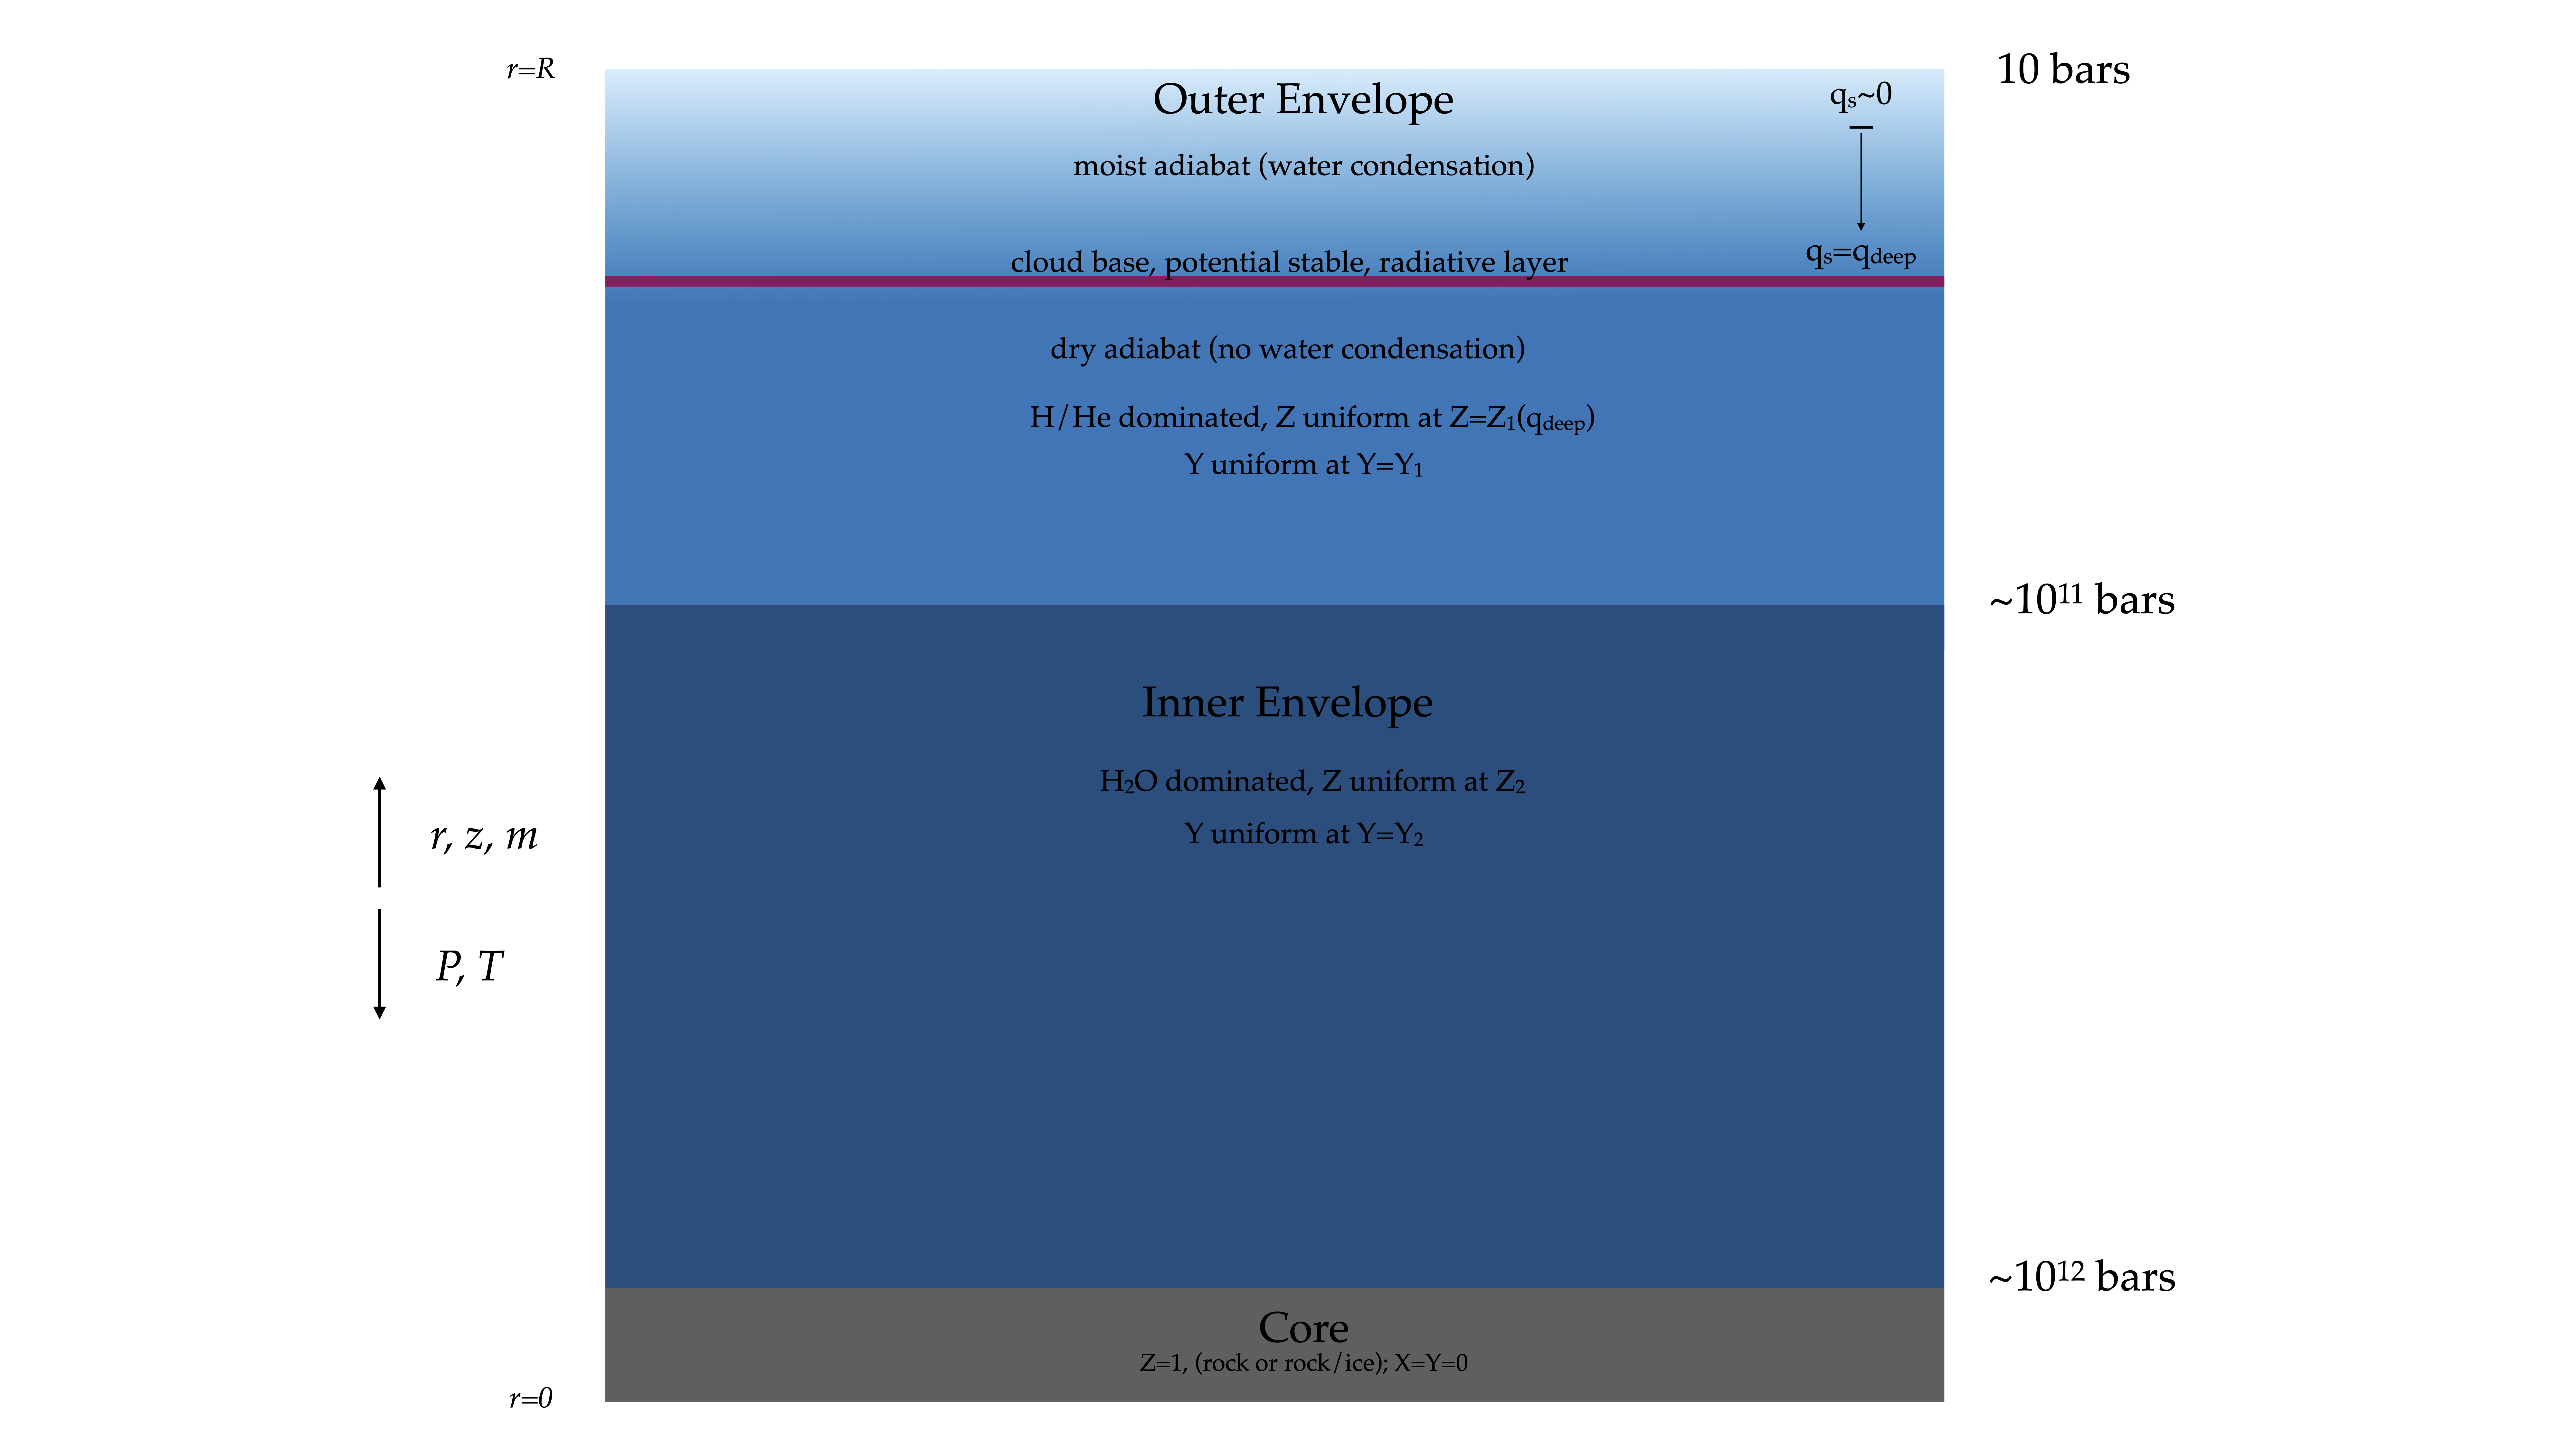
\includegraphics[width=8.0in]{figures/moist_adiabat_structure.png}
 }
\caption[Interior Structure for Moist Adiabat]
{The structure for moist adiabatic interior, allowing for condensation-inhibited convection.}
\label{fig:moist_interior}
\end{figure}


If condensation zone forms, it may be stable against convection. Convection is inhibited due to the formation of a stable condensation zone when $\alpha < 1$, where is $\alpha$ \citep{friedson_2017} is given by:

\begin{equation}
  \alpha = 1 + \xi (q_{s} L / R_{W} T_{0}) 
\end{equation}

If convection is found to be inhibited,  

At pressure where $\alpha < 1$, the cloud base of the water condensation zone forms. This thin, stable radiative layer has a temperature profile that is governed by:

\begin{equation}
	T(P) = T_{\rm top} + \int_{P_{\rm top}}^P\left(\frac{dT}{dP}\right)_{\rm rad}\,d P
\end{equation}

\section{Temperature Jump Across the Water Condensation Zone}
Letting $P_{\rm top}$ and $T_{\rm top}$ denote the pressure and temperature at the top of the stable water condensation(radiative) zone, the temperature within the radiative zone is given by
\begin{align}
T(P) &= T_{\rm top} + \int_{P_{\rm top}}^P\left(\frac{dT}{dP}\right)_{\rm rad}\,d P. \label{eq.t_of_p}
\end{align}
The radiative zone is thin under the relatively opaque conditions typical of water condensation zones in the ice giants (Leconte et al. 2017, Friedson \& Gonzales 2017). As a result our discretized model does not spatially resolve the radiative layer. Instead we treat the layer as a discontinuous increase in $T$ and water vapor mole fraction $x_{\rm vap}$. Here we derive the magnitude of the temperature jump in the limit of a thin radiative zone.

Over a thin layer, the radiative temperature gradient
\begin{align}
  \left(\frac{dT}{dP}\right)_{\rm rad}=\frac{T}{P}\nabla_{\rm rad}
  = \frac{T}{P}\times\frac{3}{16}\frac{\kappa_R P}{g}\frac{T_{\rm int}^4}{T^4}
\end{align}
is nearly constant. In this case the integral in (\ref{eq.t_of_p}) simplifies to
\begin{align}
T_{\rm base}\equiv T(P+\Delta P) &= T_{\rm top} + \left(\frac{dT}{dP}\right)_{\rm rad}\Delta P.\label{eq.t1}
\end{align}

Just as in the moist troposphere above, the local water vapor mole fraction $x_{\rm vap}$ follows the saturation value $x_{\rm vap}^{\rm sat}$ everywhere within the radiative layer, i.e.,
\begin{align}
x_{\rm vap}(P, T) &= x_{\rm vap}^{\rm sat}(P, T) = \frac{e_s(T)}{P}, \qquad P<P_{\rm base}.
\end{align}
We denote by $P_{\rm base}$ and $T_{\rm base}$ the pressure and temperature at the base of the radiative zone, which is set by the condition that $x_{\rm vap}$ has reached the deep value $x_{\rm vap}^{\rm deep}$:
\begin{align}
% x_{\rm vap}^{\rm sat}(P_{\rm top}, T_{\rm top}) &= \frac{e_s(T_{\rm top})}{P_{\rm top}} \\
x_{\rm vap}^{\rm sat}(P_{\rm base}, T_{\rm base}) &= \frac{e_s(T_{\rm base})}{P_{\rm base}}=x_{\rm vap}^{\rm deep} \\
\implies \Delta P \equiv P_{\rm base}-P_{\rm top} &= \frac{e_s(T_{\rm base})}{x_{\rm vap}^{\rm deep}} - P_{\rm top}.\label{eq.delta_p_xvap_deep}
\end{align}
(Here $e_s$ is the H$_2$O saturation vapor pressure, calculated from XXXX relation [describe what the method from thermodynamics.py actually does].)
Deeper pressures $P>P_{\rm base}$ are sub-saturated and hence no further condensation of H$_2$O takes place.
$\Delta P$ gives the extent, in pressure coordinates, of the radiative layer. Combining (\ref{eq.delta_p_xvap_deep}) and (\ref{eq.t_of_p}) yields  
\begin{align}
T_{\rm base} &= T_{\rm top} + \left(\frac{dT}{dP}\right)_{\rm rad}\left(\frac{e_s(T_{\rm base})}{x_{\rm vap}^{\rm deep}} - P_{\rm top}\right)
\end{align}
which we numerically solve for $T_{\rm base}$. Deeper temperatures are then obtained by integrating the dry adiabat $\nabla_{\rm ad}$:
\begin{align}
T(P>P_{\rm base}) &= T_{\rm base} + \int_{P_{\rm base}}^P\left(\frac{dT}{dP}\right)_{\rm ad}\,d P. \label{eq.t_of_p_deep_dry}
\end{align}
% \begin{figure}%
%     \centering
%     \subfloat[\centering The interiror structure for dry adiabat. This can also represent the situation in which the water condensation zone has eroded and the interior becomes fully convective. ]{{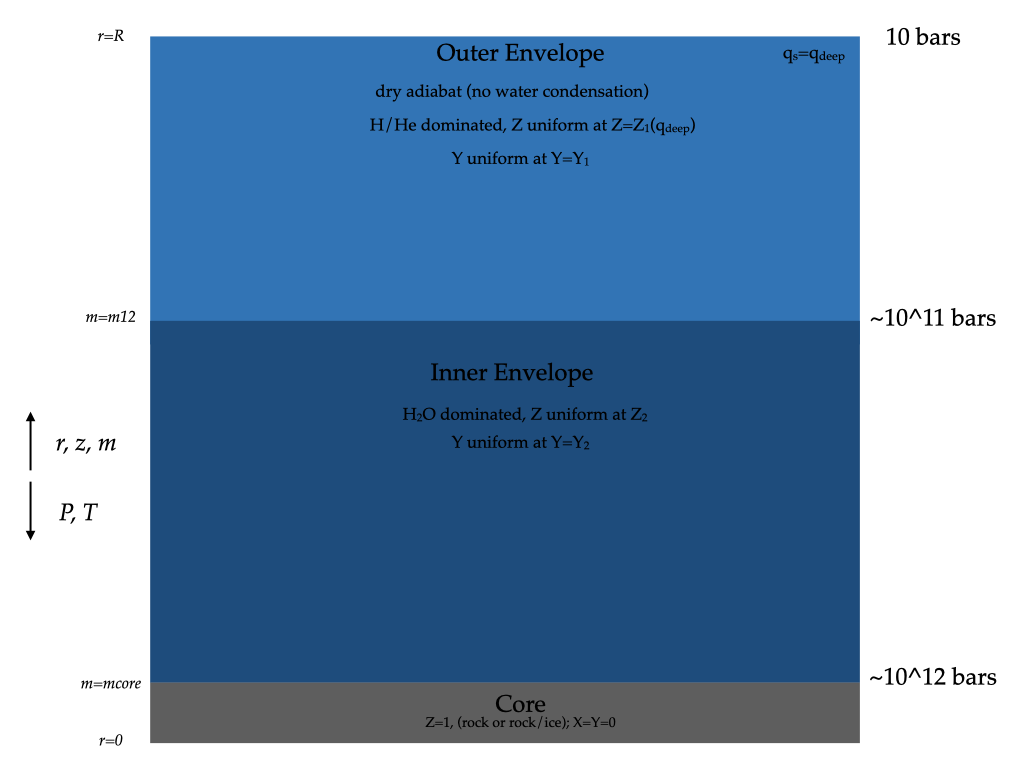
\includegraphics[width=12cm]{figures/structure_schematic_images/structure_schematic_images.001} }}%
%     \qquad
%     \subfloat[\centering The interior structure when a condensation zone has formed, creating a potentially stable, radiative layer. This represents the cloud base. It's depth decreases with a decrease in $T_{10}$. ]{{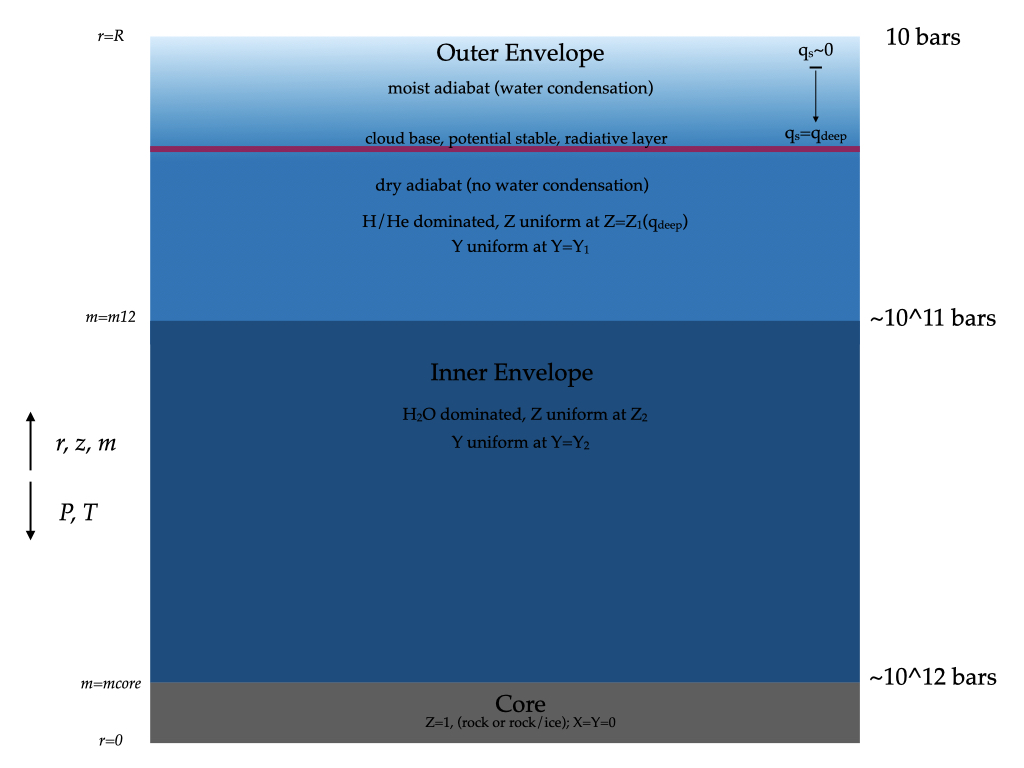
\includegraphics[width=12cm]{figures/structure_schematic_images/structure_schematic_images.002} }}%
%     \caption{Interior structure model for Uranus}%
%     \label{fig:example}%
% \end{figure}

% \begin{figure}[ht!]
%  \centerline{
%   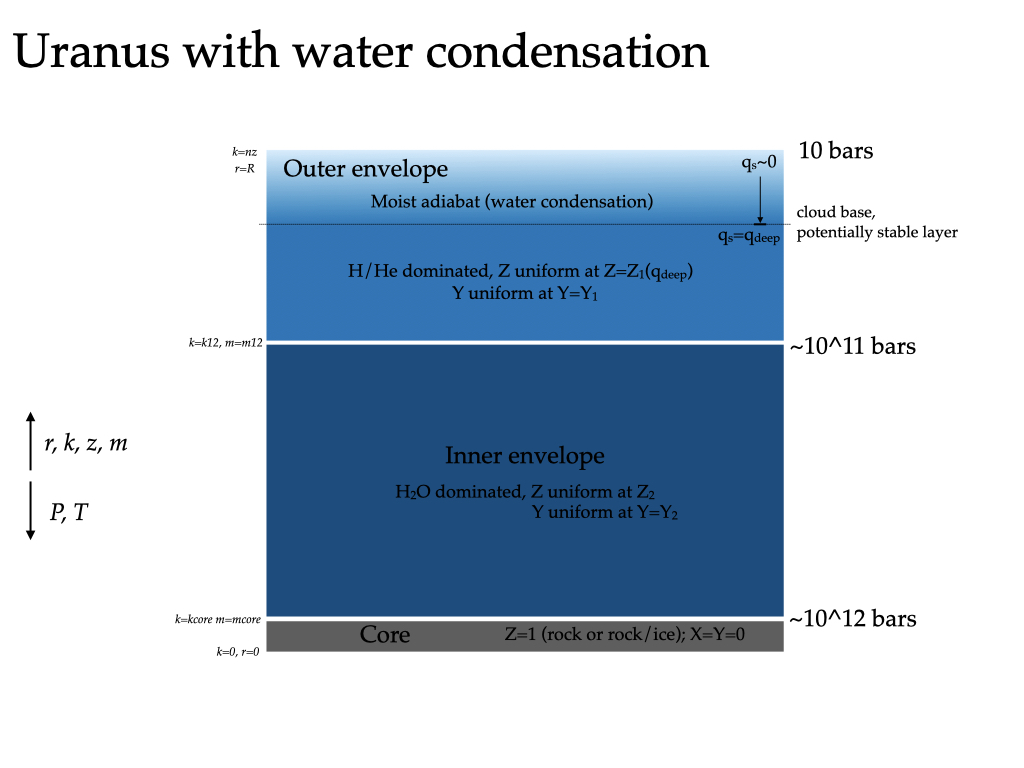
\includegraphics[width=7.0in]{figures/uranus_with_wcz_structure.001.jpeg}
%  }
% \caption[Interior Structure]
% {Model of interior structure of Uranus without condensation on the left and with condensation on the right. The dry adiabat model on the left can also represent the situation in which the water condensation zone has eroded and the interior becomes fully convective. The figure on the right shows the interior structure when a condensation zone has formed, creating a potentially stable, radiative layer. This represents the cloud base. It's depth decreases with a decrease in $T_{10}$.}
% \label{fig:uranus}
% \end{figure}

\section{Thermal Evolution of Model}
Conservation of energy relates the instantaneous luminosity profile $L(m)$ to the rate of change of specific entropy $s$ in the planet:
\begin{equation}
  \frac{dL}{dm}=-T\frac{\delta s}{\delta t}.
\end{equation}
Integrating over the mass of the planet and solving for $\delta t$ yields
\begin{equation}
\delta t=-\frac{1}{L_{\rm int}}\int_0^M T\,\delta s\,dm
\end{equation}
where $L_{\rm int}$ is the intrinsic luminosity $4\pi R^2\sigma_{\rm SB}T_{\rm int}^4$.

For our assumed ideal mixture of light elements (H/He) and heavy elements (H$_2$O) this entropy difference is simply
\begin{equation}
  \delta s = (1-Z)\delta s_{HHe} + Z\delta s_Z
\end{equation}
where in practice $\delta s_Z$ is computed in terms of the change in internal energy and density:
\begin{equation}
  T\,\delta s_Z = \delta u_Z + P\delta\left(\rho_Z^{-1}\right).
\end{equation}

\chapter{Results}

\section{Condensation-inhibited Convection}
Talk about Figure 3.1.
\begin{figure}[ht!]
 \centerline{
  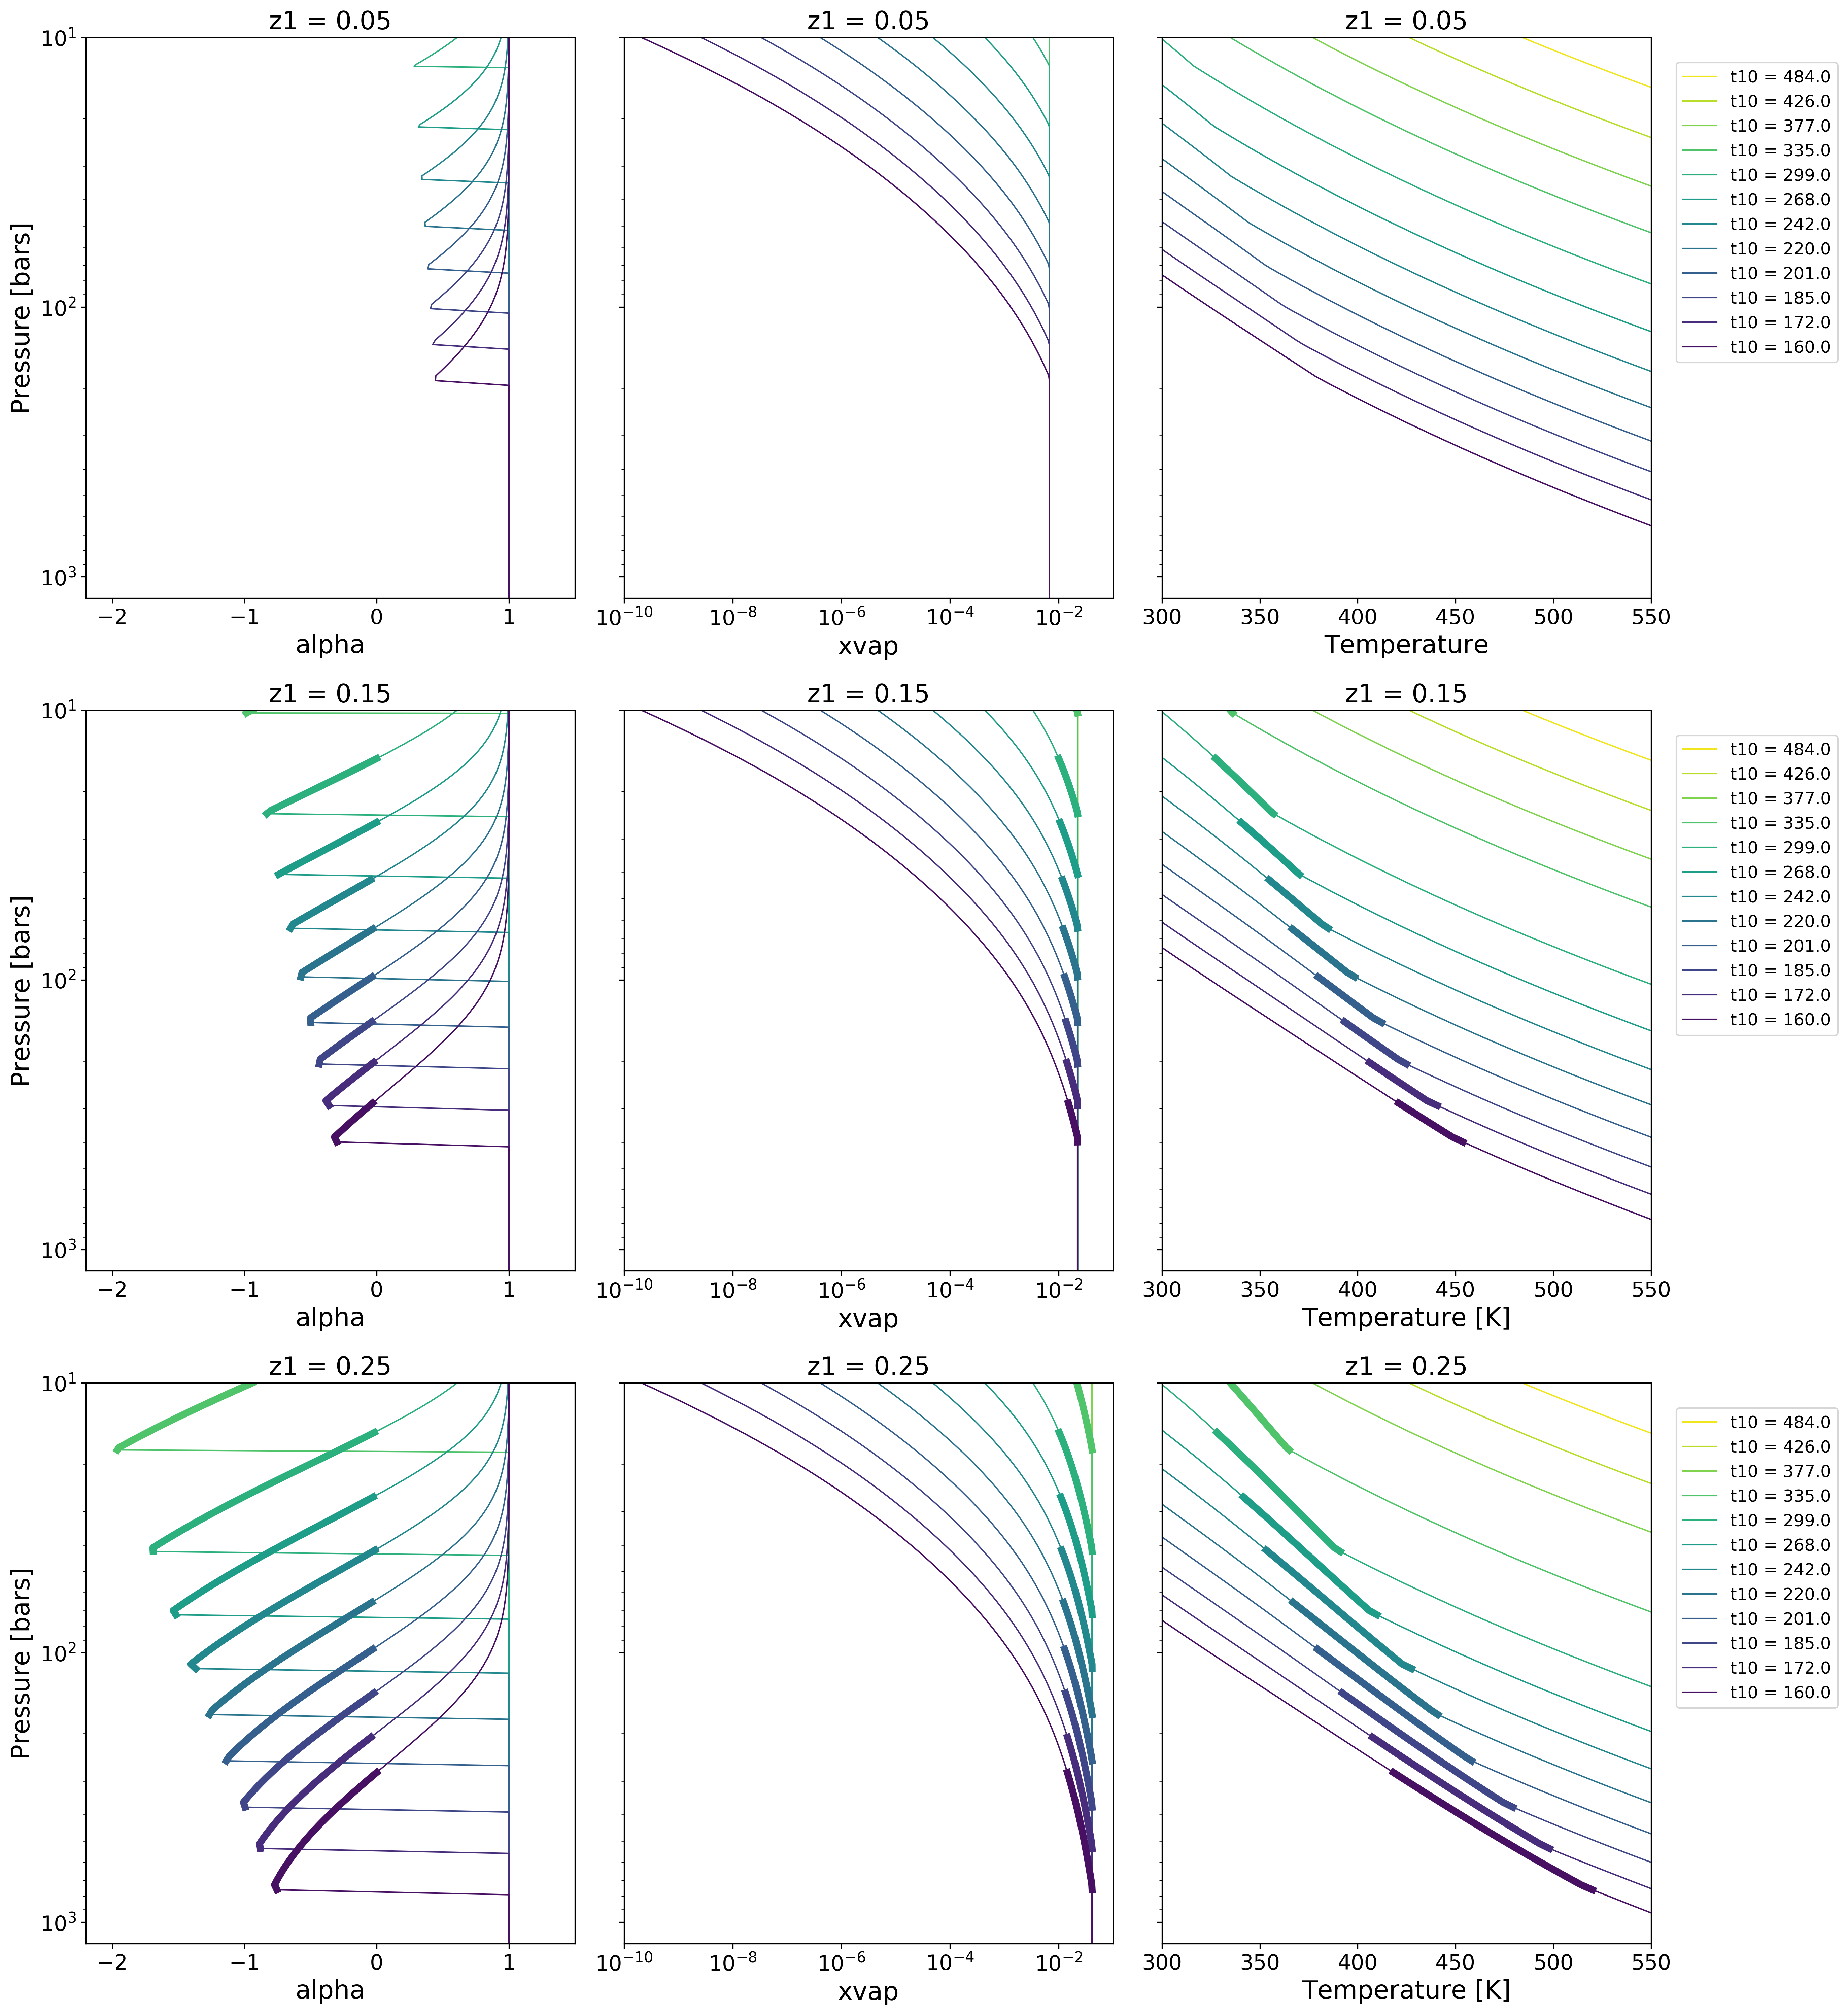
\includegraphics[width=7.0in]{figures/convection_inhibited_2.png}
 }
\caption[Inhibition of convection on Uranus]
{add description re: moist adiabat, when/where convection is inhibited and where the radiative zone base is in these plots. explain differences}
\label{fig:convection_inhibited}
\end{figure}



\section{Formation of Radiative Zone}
Talk about Figure.
\begin{figure}[ht]
 \centerline{
  \includegraphics[width=7.5in]{figures/thesis_static_radiative_layer_plots_without_grid_points.png}
 }
\caption[Inhibition of convection on Uranus]
{add description these plots. explain differences}
\label{fig:radiative}
\end{figure}


\section{Thermal Evolution of Uranus and Neptune}


\begin{figure}[ht]
 \centerline{
  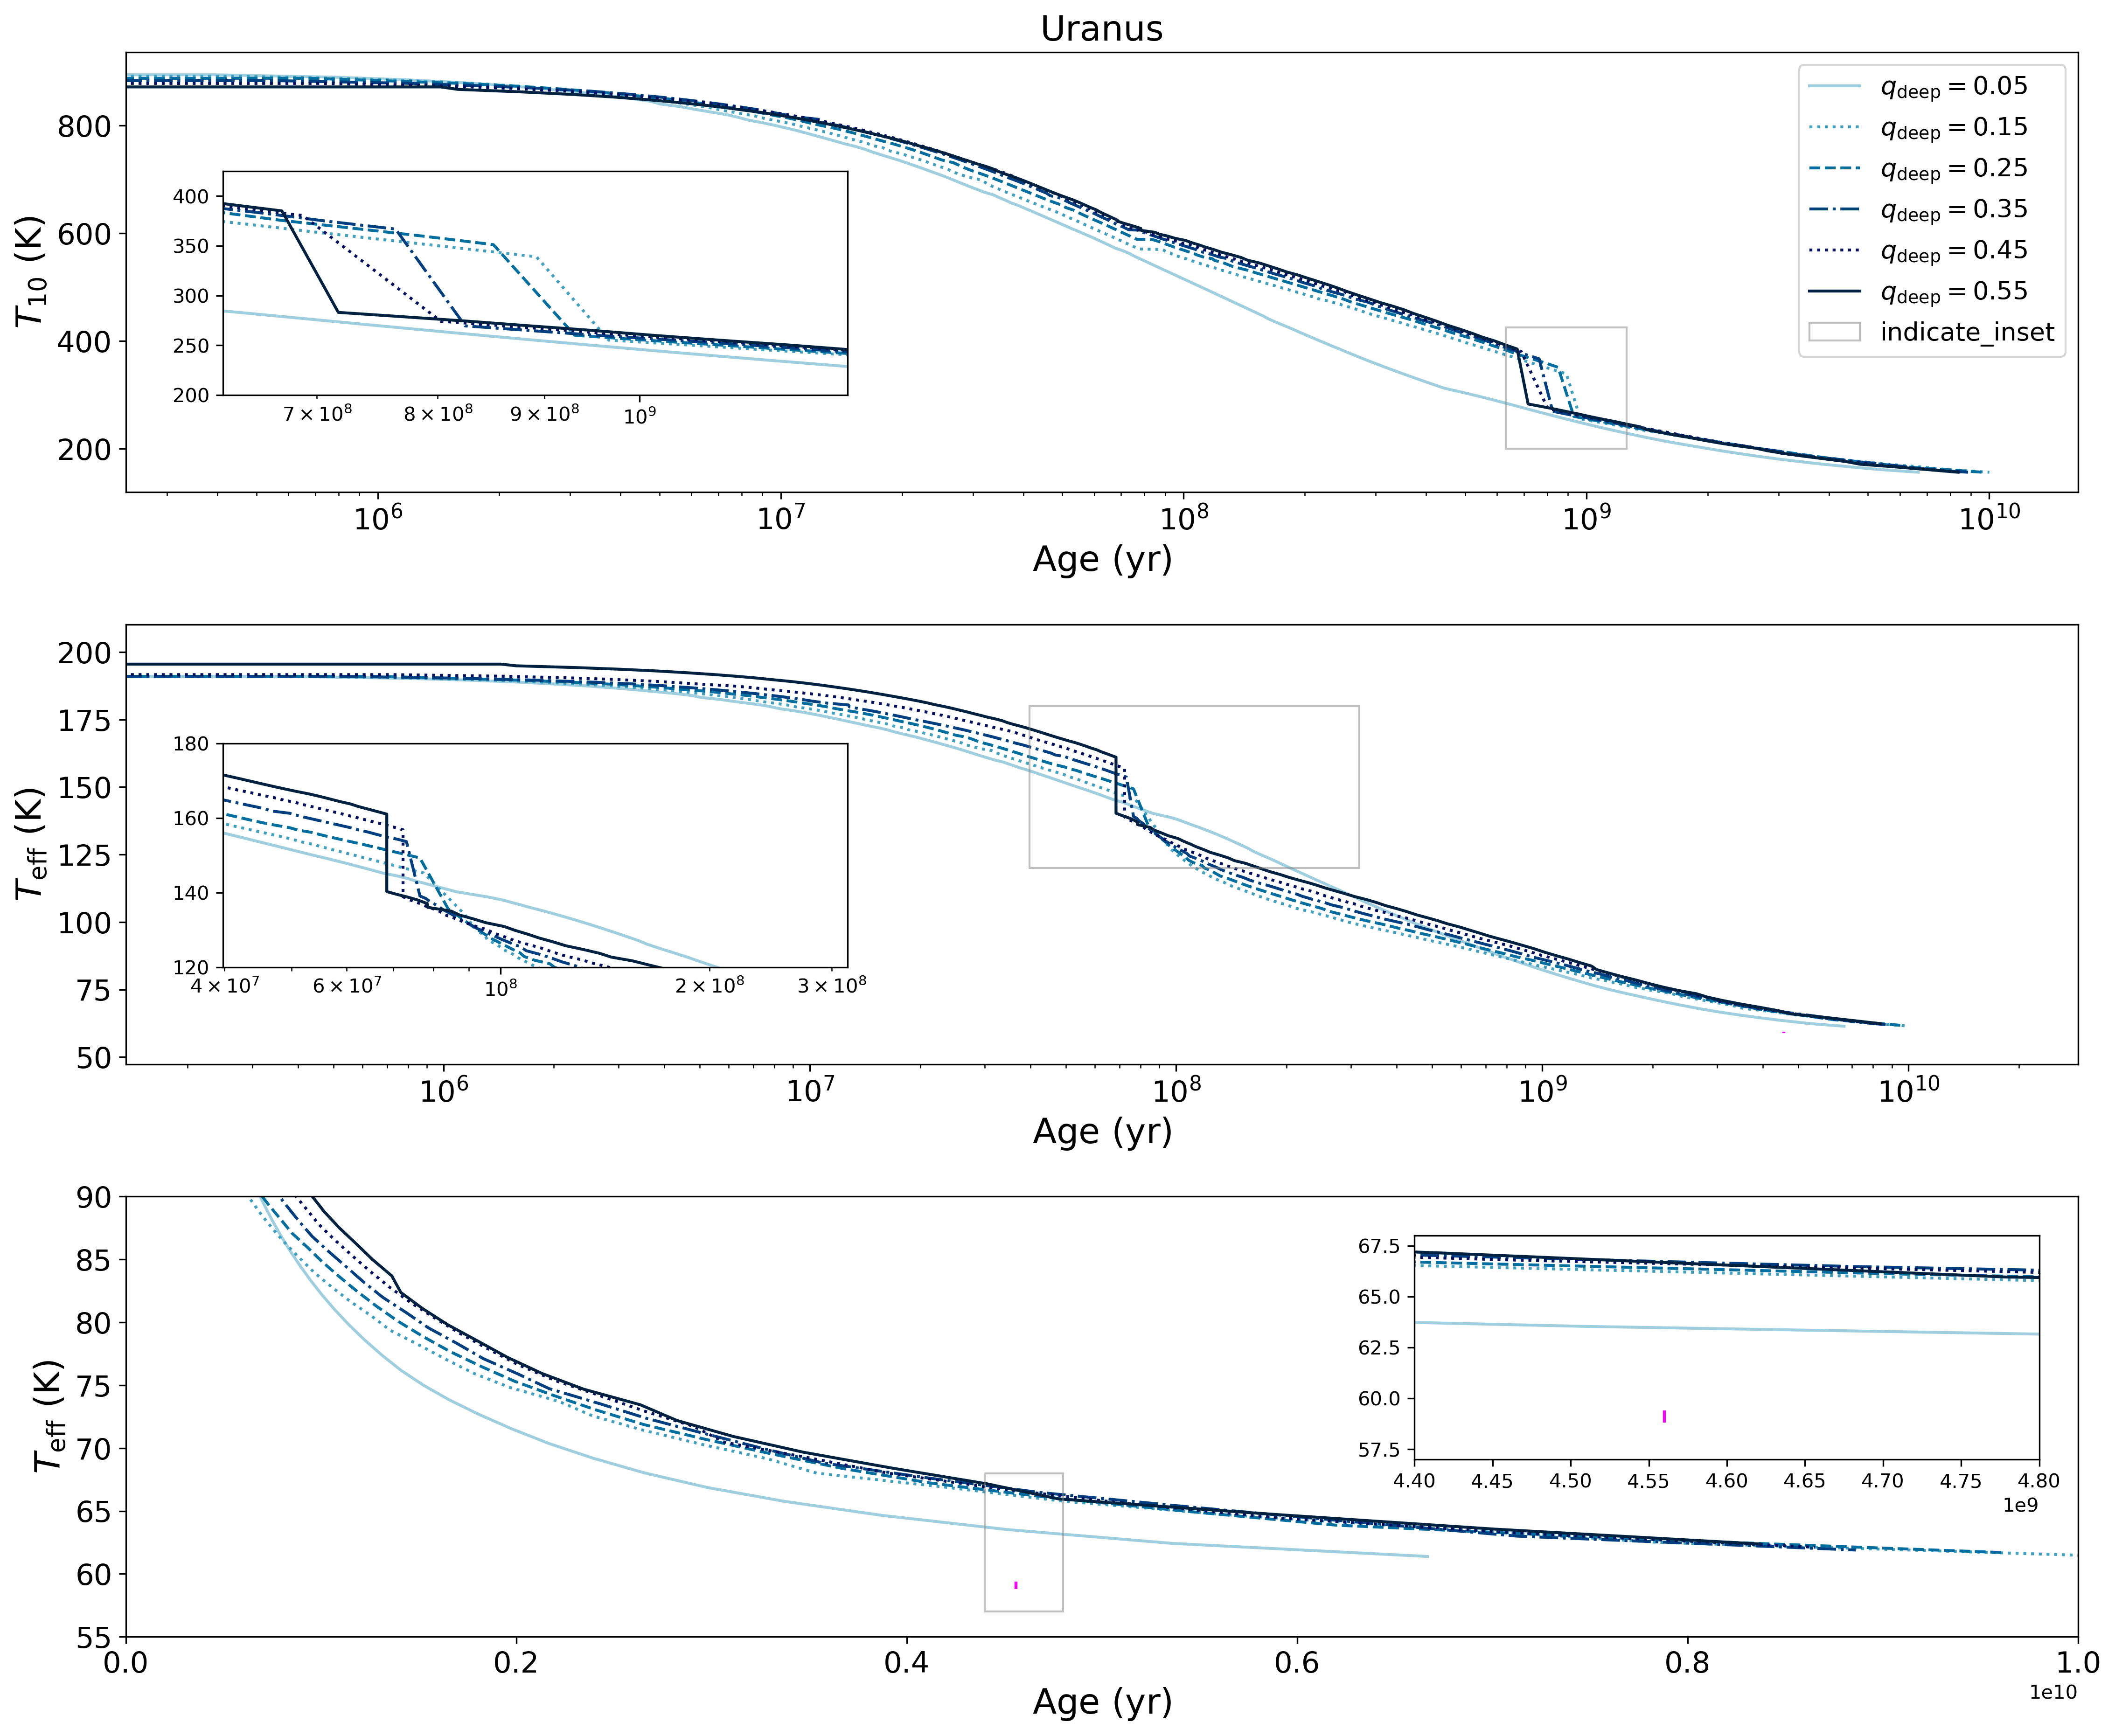
\includegraphics[scale=0.5]{figures/u_cooling_curves_nz_4096_more_qdeeps.png}
 }
\caption[Inhibition of convection on Uranus]
{add description these plots. explain differences}
\label{fig:radiative}
\end{figure}


\begin{figure}[ht]
 \centerline{
  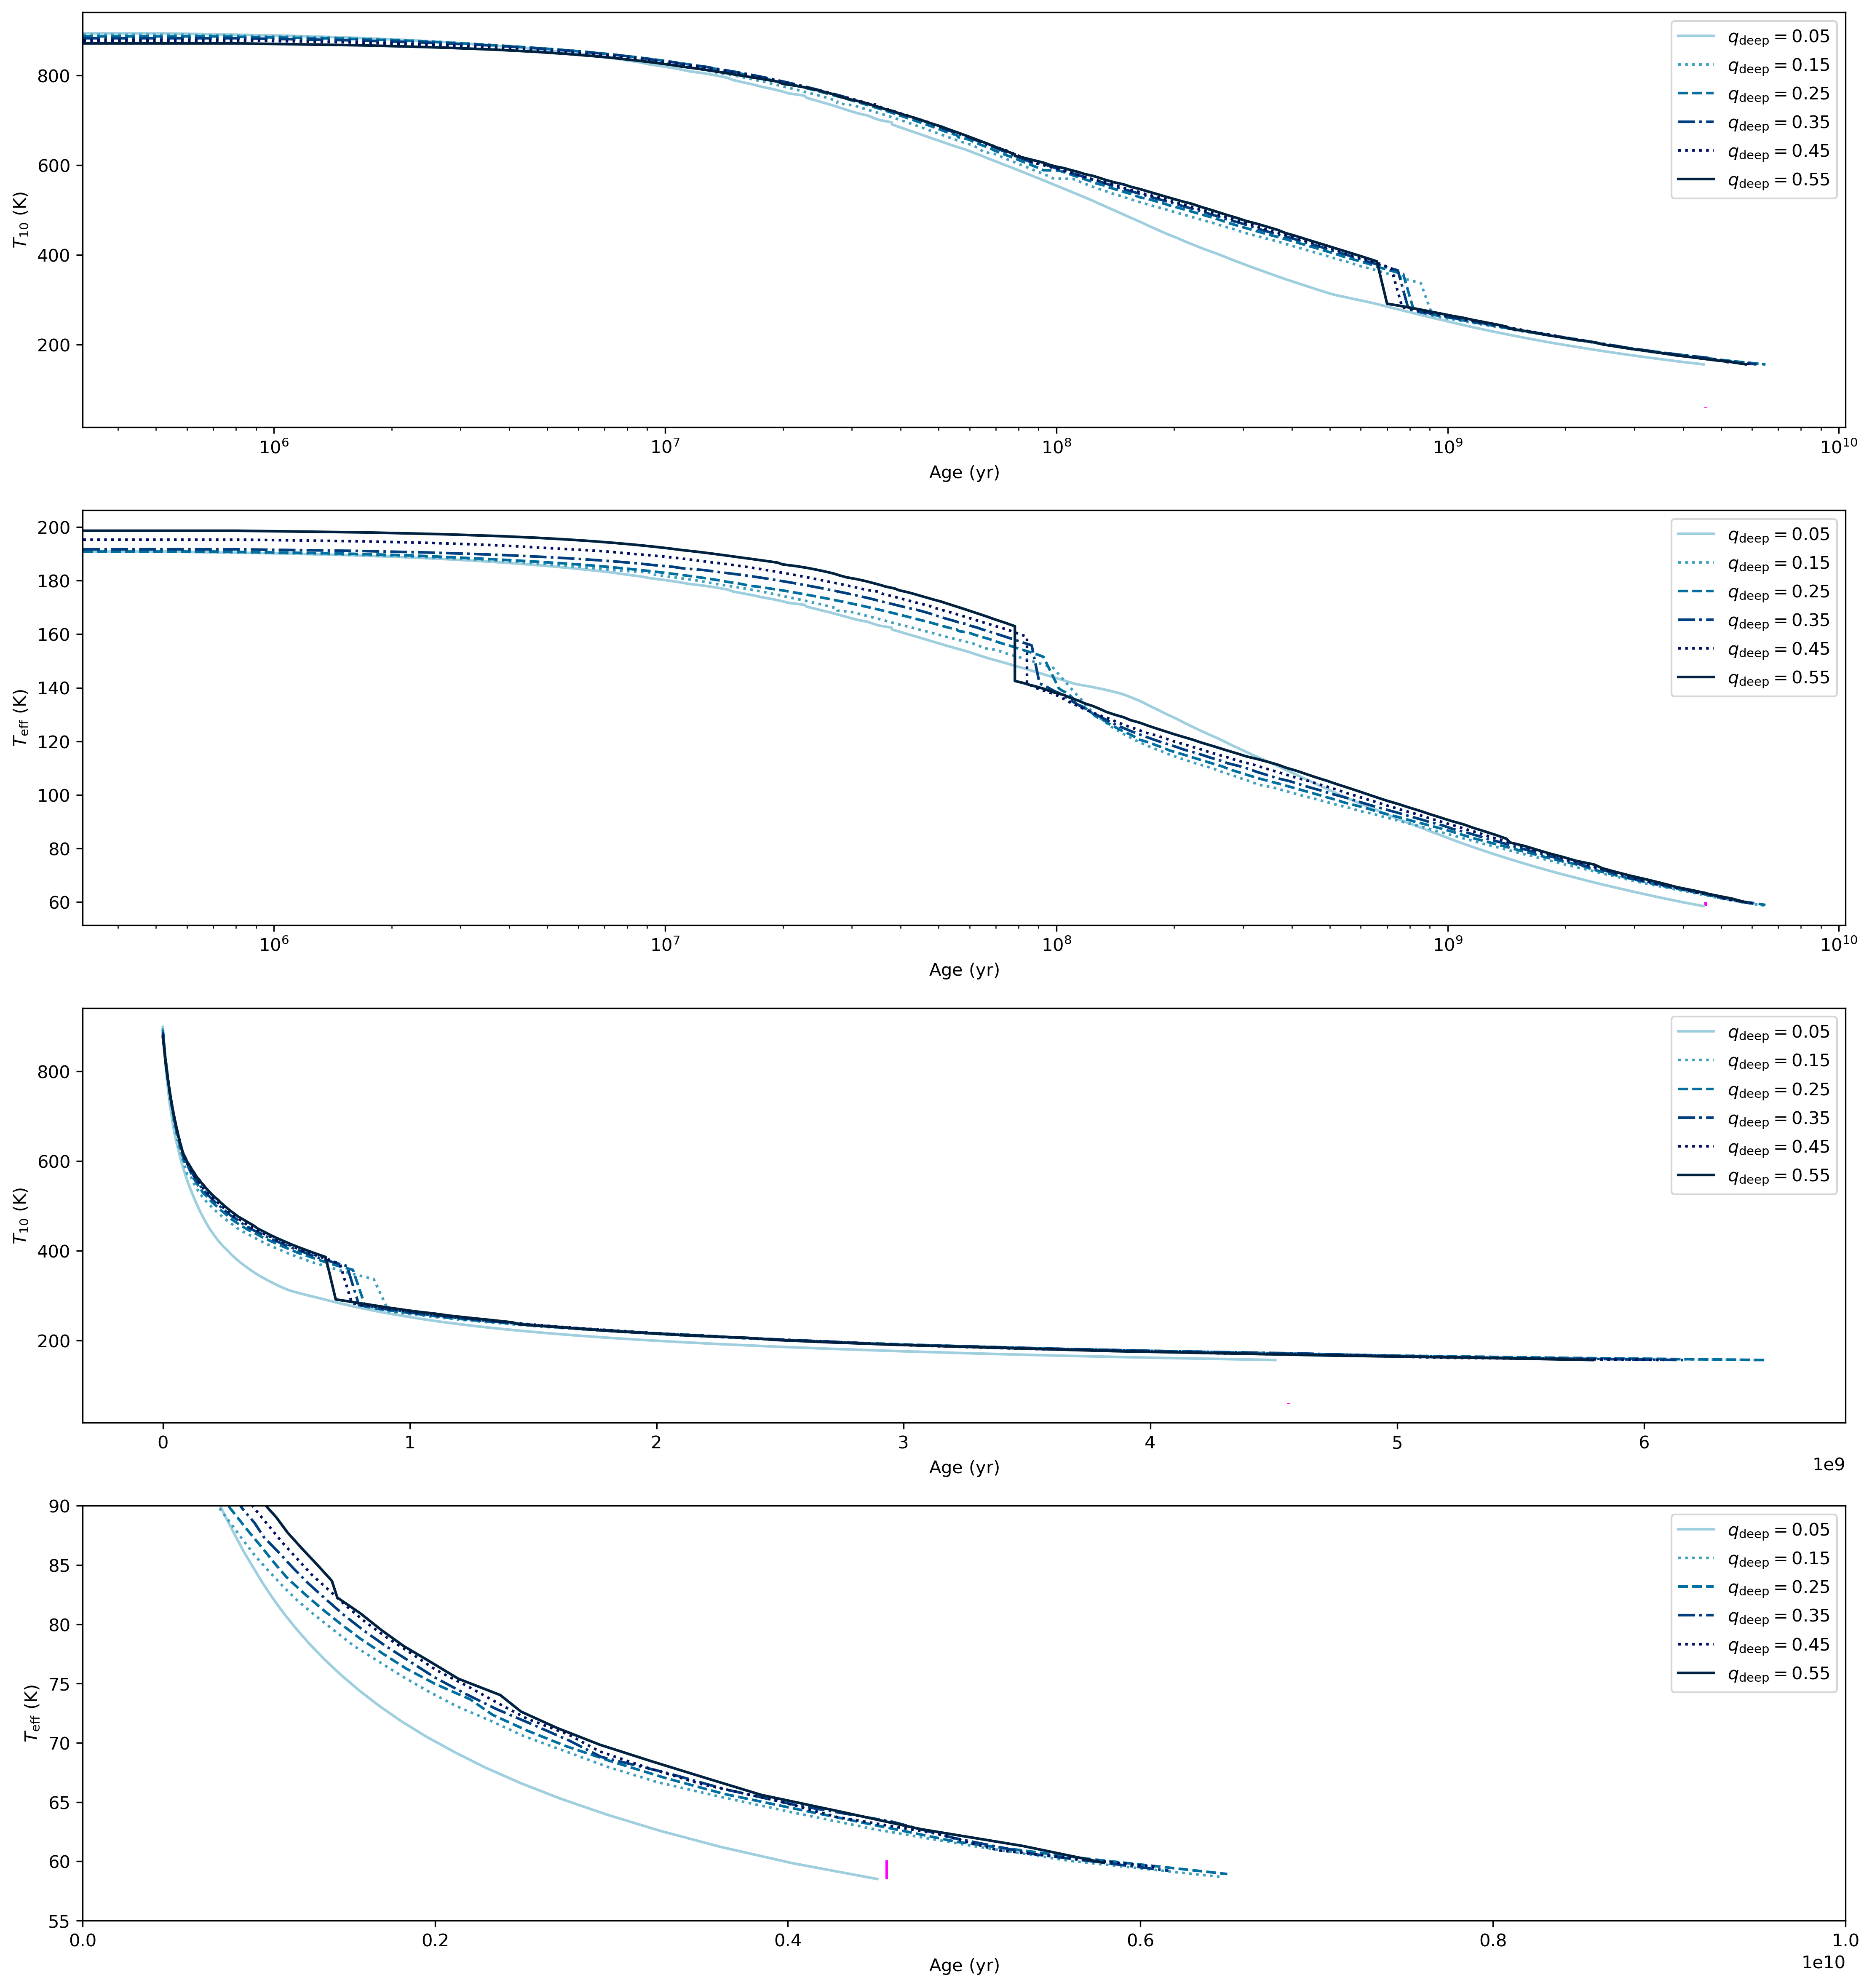
\includegraphics[scale=0.5]{figures/n_cooling_curves_nz_4096_more_qdeeps.png}
 }
\caption[Inhibition of convection on Uranus]
{add description these plots. explain differences}
\label{fig:radiative}
\end{figure}


\begin{figure}[ht]
 \centerline{
  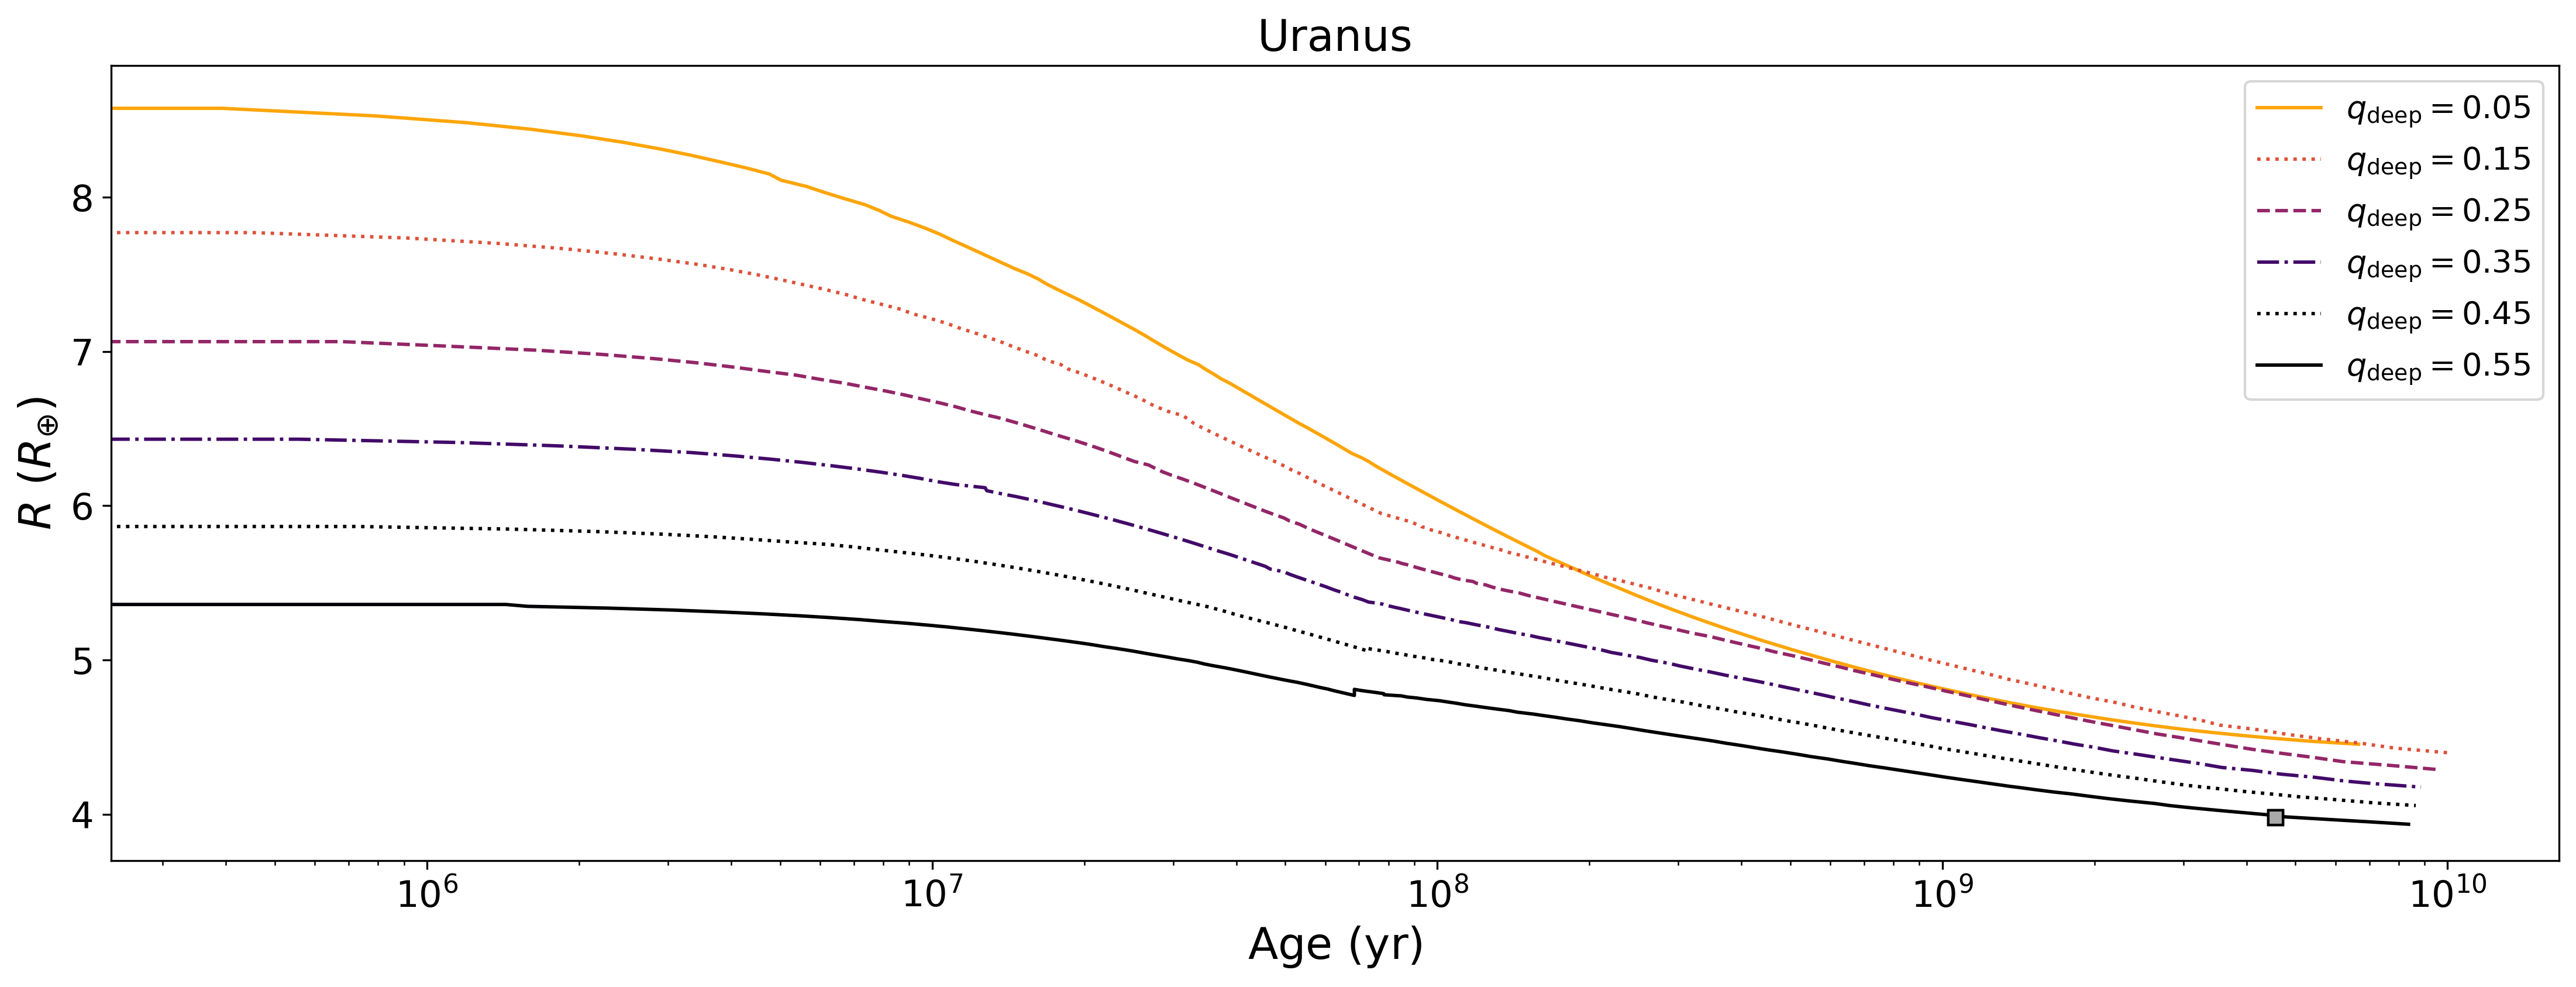
\includegraphics[scale=0.5]{figures/u_cooling_radius_nz_4096_logx_more_qdeeps.png}
 }
\caption[Inhibition of convection on Uranus]
{add description these plots. explain differences}
\label{fig:radiative}
\end{figure}



\begin{figure}[ht]
 \centerline{
  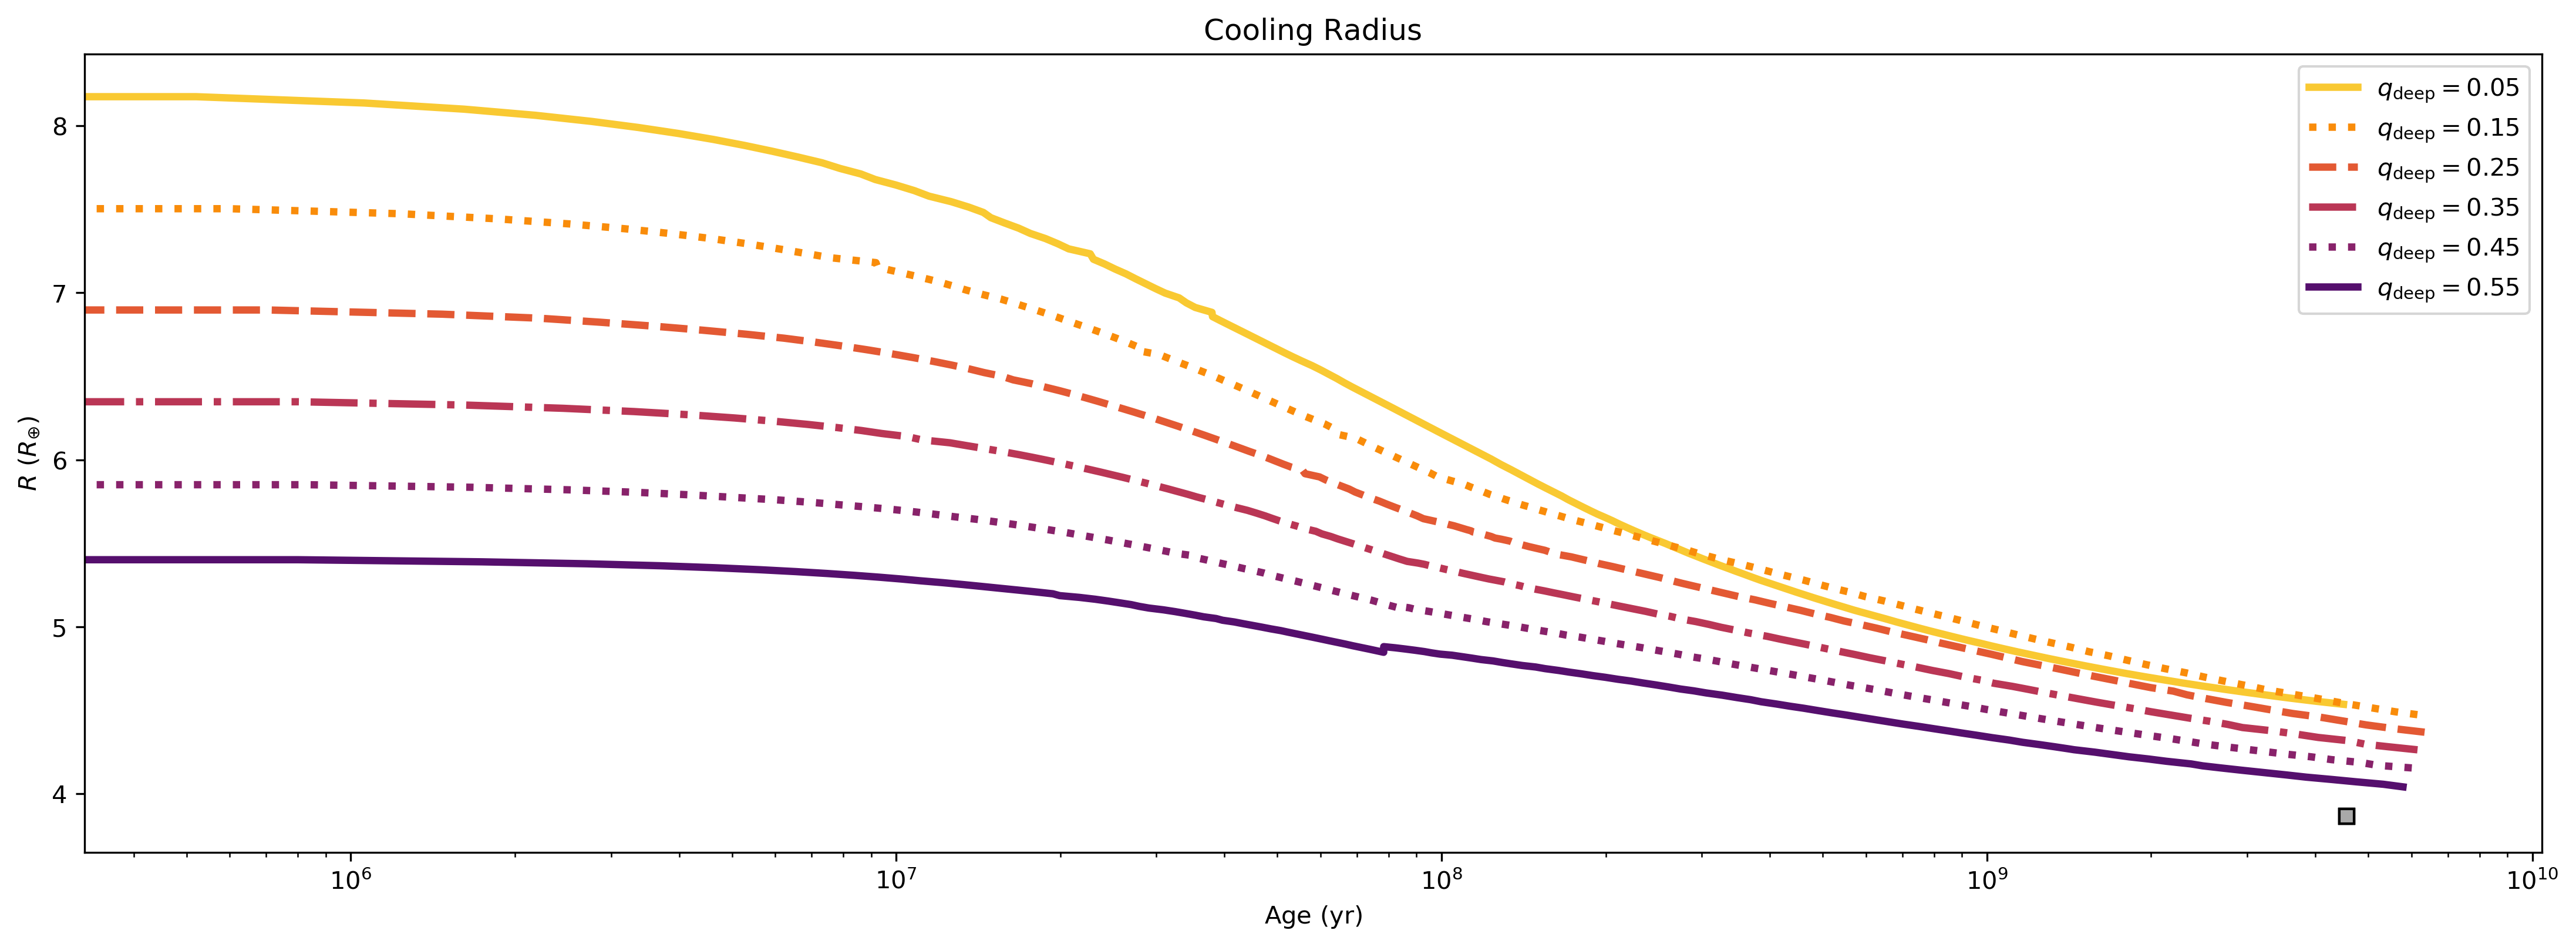
\includegraphics[scale=0.5]{figures/n_cooling_radius_nz_4096_logx.png}
 }
\caption[Inhibition of convection on Uranus]
{add description these plots. explain differences}
\label{fig:radiative}
\end{figure}




\chapter{Discussion and Conclusions}





\appendix
\chapter{Some Ancillary Stuff}

\newcommand{\newblock}{}
\bibliography{wcz_bib}


\end{document}
